\documentclass[a4paper, 12pt]{article}
\usepackage[utf8]{inputenc}
\usepackage[warn]{mathtext}
\usepackage[russian]{babel}
\usepackage[T2]{fontenc}
\usepackage[warn]{mathtext}
\usepackage{caption}

\usepackage{graphicx}
\graphicspath{ {images/} }
\usepackage{tikz}
\usepackage{pgfplots}

\usepackage{amsmath}
\usepackage{floatflt}
\usepackage[left=20mm, top=20mm, right=20mm, bottom=20mm, footskip=10mm]{geometry}

\usepackage{multicol}
\setlength{\columnsep}{2cm}

\usepackage{multicol}
\setlength{\columnsep}{2cm}
\usepackage{hyperref}
\usepackage{wrapfig}

\begin{document}
	
\begin{titlepage}
	\centering
	\vspace{5cm}
	{\scshape\LARGE Московский физико-технический институт \par}
	\vspace{4cm}
	{\scshape\Large Лабораторная работа 5.4.1 \par}
	\vspace{1cm}
	{\huge\bfseries Определение энергии $\alpha$-частиц по велечине их пробега в воздухе\par}
	\vspace{1cm}
	\vfill
\begin{flushright}
	{\large выполнил студент 924 группы ФОПФ}\par
	\vspace{0.3cm}
	{\LARGE Панферов Андрей}
\end{flushright}
	

	\vfill

% Bottom of the page
	Долгопрудный, 2021 г.
\end{titlepage}

\paragraph*{Цель работы:} Измерить пробег альфа-частиц в воздухе с помощью ионизационной камеры.
\section*{Описание установки}
\paragraph*{Ионизационная камера}
	
	Ионизационная камера --- прибор для количественного измерения
	ионизации, произведенной заряженными частицами при прохождении
	через газ. Камера представляет собой наполненный газом сосуд с двумя электродами (схема камеры приведена на рис. \ref{ris Ion}). 
	
	Заполняющий сосуд газ сам по себе не проводит электрический ток, возникает он только при прохождении быстрой заряженной частицы, которая рождает в газе на своем пути ионы.
	
	Поместим на торец внутреннего электрода источник
	ионизирующего излучения (в нашем случае это источник
	альфа-частиц $ ^{239}_{94} $Pu), заполним объем камеры воздухом и начнем
	постепенно увеличивать разность потенциалов между электродами. Ток, протекающий через камеру, вначале будет резко возрастать, а затем, начиная с некоторого напряжения $ V_0 $, станет постоянным, т. е. "<выйдет на плато">.  Предельный ток $ I_0 $ будет равен $ I_0 = n_0e $,
	где $ n_0 $ --- число пар ионов, образуемых в секунду в объеме камеры, а $ e $ --- заряд электрона.
	
	\begin{wrapfigure}[16]{l}{0.37\linewidth}
		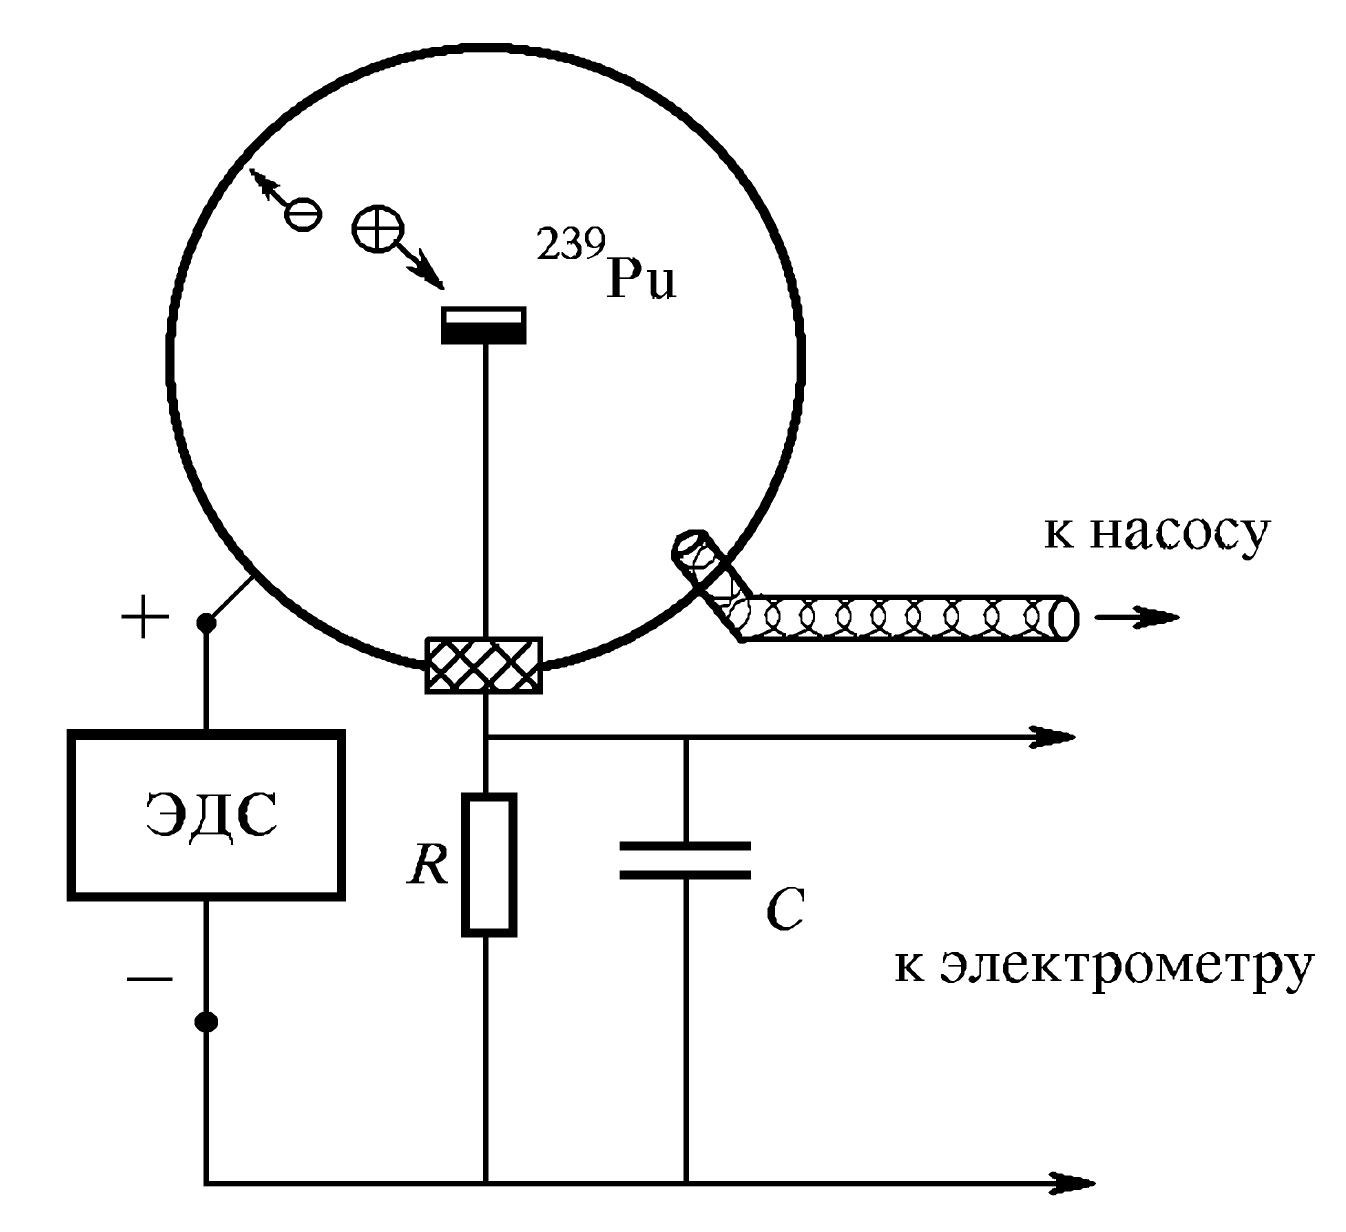
\includegraphics[width=\linewidth]{Ion}
		\caption{Схема устройства ионизационной камера}
		\label{ris Ion}
	\end{wrapfigure}
	
	Прохождение тока через камеру регистрируется посредством измерения напряжения на включенном в цепь камеры сопротивлении $ R $.
	Так как средняя энергия ионизации атомов воздуха составляет около 30 эВ, то альфа-частица с энергией 3 МэВ образует на своем пути около $ 10^5 $ электронов, им соответствует заряд $1,6 \cdot 10^{-14} $ Кл. Чтобы
	столь малое количество заряда, создаваемое проходящей через камеру одной альфа-частицей, вызывало измеряемое напряжение, емкость $ C $
	должна быть мала.
	
	При изменении давления в камере ионизационный ток меняется сначала линейно, а потом выходит на насыщение. При небольших давлениях газа
	альфа-частицы передают часть энергии стенкам камеры. По достижении
	давления $ P_0 $ все они заканчивают свой пробег внутри газа, и дальнейшее возрастание тока прекращается.
	
	В данной работе измерение пробега альфа-частицы проводится по величине тока ионизации в сферической камере. Вакуумная установка содержит кран и манометр. Она позволяет изменять давление в камере от атмосферного до 10 мм рт. ст.
	Величина тока ионизации измеряется электрометром, состоящим из
	нескольких стандартных микросхем, по величине падения напряжения
	на сопротивлении $ R $ = 100 МОм ($ C = 10^{-8} $ Фарад, так что $ RC $ = 1 с).
	Значение измеряемого ионизационного тока (в пикоамперах) высвечивается на цифровом табло.
	
	\newpage
	
	\section*{Выполнение работы}
	\begin{enumerate}
	
		
		\item Включив питание установки, измерим при атмосферном давлении $ P_a = 102,6 $ кПа = 769,9~Торр (измеренном барометром) ток $ I_a = 820 $ пА. Температура $ T = 298 $ К.
		\vspace{0.1cm}
		
		\begin{minipage}{0.45\textwidth}
		 После этого откачаем воздух из камеры до давления порядка $ \approx 10 $ Торр и снимем зависимость тока от давления, запуская воздух в камеру.
		
		(Погрешность давления оценим как цену деления --- $ \sigma_P = 5 $ Торр, погрешность $ \sigma_I = 3 $ пФ. Результаты измерения занесем в Таблицу \ref{table:current}. Построим График \ref{graph:current} полученной зависимости)
		
		\begin{center}
            \begin{tikzpicture}[scale=0.8]
                \label{graph:current}
                \begin{axis}[
                    	axis lines = middle,
                    	xlabel = {$P$, mmHg},
                        ylabel = {$I$, pA},
                    	ylabel style={red, scale=1},
                        xlabel style={red, scale=1},
                    	title={Зависимость тока в камере от давления},
                    	table/col sep=semicolon,
                    	xmin = 0,
                    	ymin = 0,
                    ]
            	    \addplot +[blue, only marks] table[x=P2, y=I]{data.txt};
            	    \addplot[color=red, domain=60:610]{1.86 * x - 80};
            	    \addplot[color=red, domain=510:760]{-0.262 * x + 1150};
            	    \addplot[thick, samples=50, smooth,domain=0:1000,grey] coordinates {(578,0)(578,1000)};
            	\end{axis}
            \end{tikzpicture}
        \end{center}
		
		
		\end{minipage}
		\hspace{0.1cm}
		\begin{minipage}{0.5\textwidth}
		    \captionof{table}{Зависимость тока в камере от давления}
		    \label{table:current}
		    \centering
                \begin{tabular}{|r|r|r|r|}
                \hline
                \multicolumn{1}{|l|}{$P$, mmHg} & \multicolumn{1}{l|}{$I$, pA} & \multicolumn{1}{l|}{$P$, mmHg} & \multicolumn{1}{l|}{$I$, pA} \\ \hline
                700                                 & 945                          & 150                                & 302                          \\ \hline
                675                                 & 952                          & 125                                & 253                          \\ \hline
                625                                 & 969                          & 100                                & 218                          \\ \hline
                575                                 & 982                          & 75                                 & 172                          \\ \hline
                550                                 & 990                          & 50                                 & 135                          \\ \hline
                530                                 & 990                          & 25                                 & 93                           \\ \hline
                525                                 & 982                          &                                    &                              \\ \hline
                500                                 & 975                          &                                    &                              \\ \hline
                475                                 & 925                          &                                    &                              \\ \hline
                450                                 & 895                          &                                    &                              \\ \hline
                425                                 & 835                          &                                    &                              \\ \hline
                400                                 & 785                          &                                    &                              \\ \hline
                375                                 & 721                          &                                    &                              \\ \hline
                350                                 & 680                          &                                    &                              \\ \hline
                325                                 & 615                          &                                    &                              \\ \hline
                300                                 & 582                          &                                    &                              \\ \hline
                275                                 & 520                          &                                    &                              \\ \hline
                250                                 & 484                          &                                    &                              \\ \hline
                225                                 & 420                          &                                    &                              \\ \hline
                200                                 & 393                          &                                    &                              \\ \hline
                175                                 & 337                          &                                    &                              \\ \hline
                \end{tabular}
		\end{minipage}
		
		
	\item На график нанесем прямые соответствующие линейным участкам зависимости.
	По их пересечению оценим точку перелома:
	$$P_{0} = 580 \pm 10 \text{мм рт. ст.}$$
	
	Приведем данные к нормальным температуре и давлению для нахождения пробега частицы в нормальных условиях:
	$$R_l = 5\text{см, } \implies R_{norm} = R_l\frac{P_0T_{norm}}{P_{norm}T_0} = 3.75 \pm 0.05\text{см, }$$
	
	Из пробега по имперической формуле найдем энергию частиц:
	
	$$R = 0.32 E^{3/2} \implies E = 5.2 \pm 0.1\text{МэВ}$$

	\end{enumerate}
	
	\section*{Вывод}
	В работе был измерен пробег альфа-частиц от $ ^{239}  $Pu с помощью ионизационной камеры. По полученным данным была определена энергия $\alpha$-частиц.
	
	При работе с ионизационной камерой пробег и энергия получились близкими к ожидаемым: $5.2\pm0.1$МэВ против табличных $5.244$МэВ.  
	
	Если плотность бумаги равна $ 1,2 \; \text{г/см}^3 $, следовательно, лист бумаги толщины $~l~\geq~R'/\rho \hm{=}36, 6 $~мкм не пропустит альфа-частицы от $ ^{239}  $Pu.
\end{document}